\documentclass{IMTexam}

\usepackage{IMTtikz}
\DeclareSIUnit{\atm}{atm}
\DeclareSIUnit{\calorie}{cal}
\usepackage{mhchem}

%\mmaDefineMathReplacement[≤]{<=}{\leqslant}
%\mmaDefineMathReplacement[≥]{>=}{\geqslant}
%\mmaDefineMathReplacement[≠]{!=}{\neq}
%\mmaDefineMathReplacement[→]{->}{\to}[2]
%\mmaDefineMathReplacement[⧴]{:>}{:\hspace{-.2em}\to}[2]
%\mmaDefineMathReplacement{∉}{\notin}
%\mmaDefineMathReplacement{∞}{\infty}
%\mmaDefineMathReplacement{𝕕}{\mathbbm{d}}
%\mmaSet{
%  morefv={gobble=2},
%  linklocaluri=mma/symbol/definition:#1,
%  morecellgraphics={yoffset=1.9ex}
%}
\usepackage{listings,xcolor}

\lstset{language=Mathematica}
\lstset{basicstyle={\sffamily\footnotesize},
  numbers=left,
  numberstyle=\tiny\color{gray},
  numbersep=5pt,
  breaklines=true,
  captionpos={t},
  frame={lines},
  rulecolor=\color{black},
  framerule=0.5pt,
  columns=flexible,
  tabsize=2
}


\givecredits
\author{Isabella B. \& Joel B. \& Jonathan B.}
\USPN{118010773}
\lecture{Química II}
\examname{Prova I}
\hwtype{Resolução}
\lcode{}
\date{06 de junho}

\begin{document}
    \maketitle

    \paragraph{Utilize caso achar necessário:}
    \[ R = \SI{8,3145}{\joule\per\kelvin\per\mole}, R = \SI{0,082057}{\liter\atm\per\kelvin\per\mole},
    R=\SI{82,05745}{\centi\meter\cubed\atm\per\kelvin\per\mole}, R=\SI{1,897}{\calorie\per\kelvin\per\mole}\]
    Justifique sua resposta e mostre as etapas de cálculo. Não esqueça das unidades!

    \begin{questions}
        \question A equação de estado $P(Vm – b) = RT$ é adotada, às vezes, em
        cálculos aproximados envolvendo gases reais. Admitindo que existam gases
        que obedecem rigorosamente a essa equação.

        \begin{parts}
            \part  É possível liquefazer tais gases? Justifique seu raciocínio.
            Sugestão: considere a similaridade da equação com a equação de van
            der Waals.
            \begin{solution}
                A equação proposta é só a equação de van der Waals sem o
                parâmetro a, que corrige valores para levar em conta interações
                intermoleculares atrativas. Essas interações são as resposáveis
                pela liquefação, então não se espera que os gases se liquefaçam.

                Em particular, as isotermas da equação proposta são só uma
                translação por b das isotermas de gases ideais. A informação
                sobre liquefação contida na equação de van der Waals (regiões
                físicamente ``incorretas" onde P e V aumentam juntos) só existe
                pelo seu caráter cúbico, mas as isotermas de gases ideais e da
                equação proposta são lineares. Logo, não devem conter informação
                sobre ou prever liquefação.
            \end{solution}

        \end{parts}
        \question A \SI{273}{\kelvin}, o argônio tem os seguintes coeficientes
        do virial: $B = \SI{-21,7}{\centi\meter\cubed\per\mole}$ e
        $C=\SI{1200}{\centi\meter\tothe{6}\per\mole\squared}$. Admitindo que a
        lei dos gases perfeitos seja suficientemente exata para estimar o
        segundo e terceiro termos da expansão (ou seja, use a lei dos gases
        perfeitos em caso de necessidade):

        \begin{parts}
            \part calcule o fator de compressibilidade do argônio a \SI{100}{\atm} e
            \SI{273}{\kelvin}. Sugestão: Obtenha uma expressão para $Z$ em função de $P$ com $B,
            C$ e $T$ constantes.

            \begin{solution}
                Sendo $Z=V_m/V_m^0$, $V_m^0=RT/P$, devemos encontrar $V_m(P,T)$,
                dessa forma

                \begin{align*}
                    P&=RT\del{\dfrac{1}{V_m}+\dfrac{B}{V_m^2}+\dfrac{C}{V_m^3}}\\
                    V_m^3&=\dfrac{RT}{P}\del{V_m^2+B\,V_m+C}\\
                    \intertext{sendo $\int\od{}{x}f(x)\dif x=f(x)$, temos que}
                    \int \dod{\sbr{V_m^3}}{V_m}\dif V_m&=\int \dod{}{V_m}\sbr{\dfrac{RT}{P}\del{V_m^2+B\,V_m}+\underbrace{\dfrac{RT}{P}C}_{=\beta}} \dif V_m\\
                    \int 3V_m^2\dif V_m &=\int \dfrac{RT}{P}\del{2V_m+B} \dif V_m\\
                    \intertext{e, pela linearidade da integral, temos}
                    \int V_m^2- \underbrace{\dfrac{RT}{3P}}_{=\alpha}\del{2V_m+B} \dif V_m &=\dfrac{\beta}{3}=\dfrac{RT}{3P}\,C\\
                    \int V_m^2- 2\alpha\,V_m+\alpha^2+\alpha\,B-\alpha^2 \dif V_m&=\alpha\,C\\
                    \int \del{V_m-\alpha}^2+\alpha\,B-\alpha^2\dif V_m &=\alpha\,C\\
                    \intertext{tomando $u=V_m-\alpha\implies \dif V_m=\dif u$, temos}
                    \int u^2+\alpha\,B-\alpha^2\dif u &=\alpha\,C\\
                    \dfrac{1}{3}u^3+\underbrace{\del{\alpha\,B-\alpha^2}}_{=\gamma}u &=\alpha\,C\\
                \end{align*}
                realizando os próximos cálculos com o Mathematica (vide \ref{code:math}), substituímos as
                variáveis, resolvendo para $V$ e tomamos a razão de
                $Z=V_m/V_m^0=\num{137.661}$.

            \end{solution}

            \part Explique como o fator de compressibilidade varia com a
            temperatura. Faça um esboço indicando o comportamento de $Z$ acima e
            abaixo da temperatura de Boyle (TB), identificando também essa
            temperatura no esboço.

            \begin{solution}
                Quanto menor a temperatura maior a tendência de forças
                interatômicas se sobressaírem ─ já que moléculas mais inertes
                tendem a interagir mais entre si ─, provocando efeitos diferentes
                daqueles estimados pela lei dos gases ideais.

                Como a temperatura de Boyle marca o ponto onde as forças se
                cancelam, temos que para temperaturas menores do que esta as
                forças de atração devem vencer e, portanto, $Z<1$ (volume real
                menor do que o esperado), e vice-versa.

                \begin{center}
                    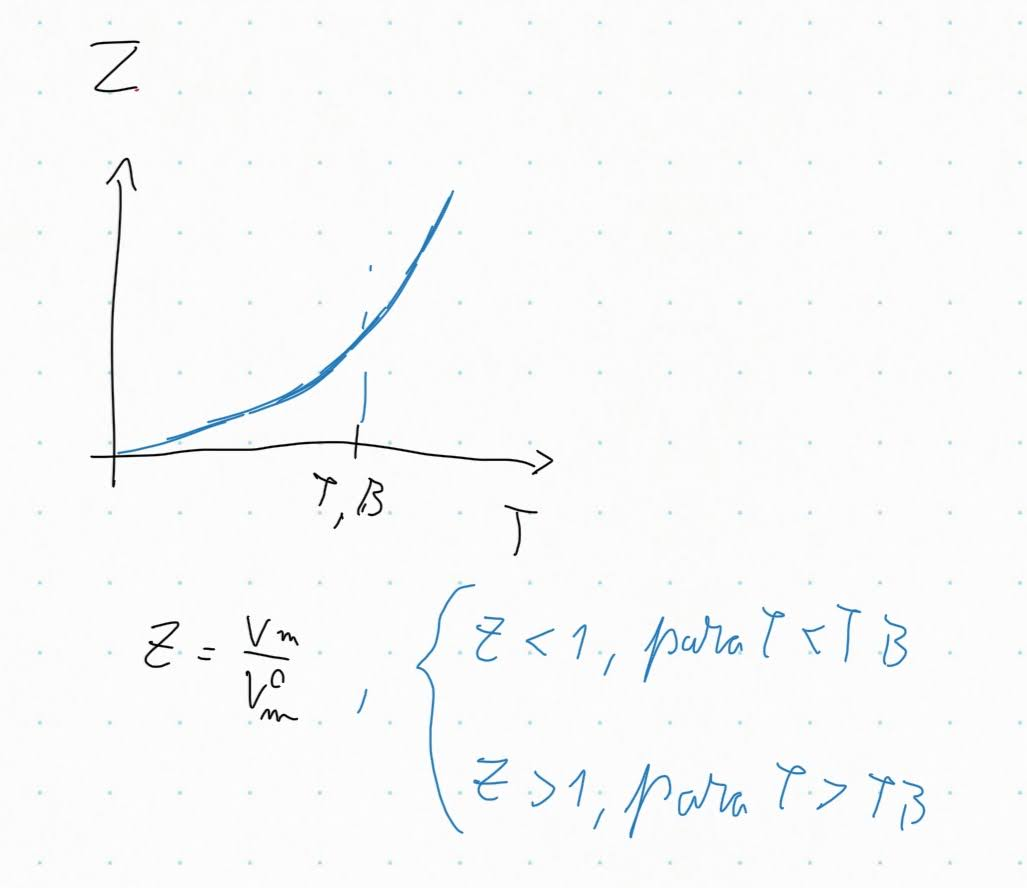
\includegraphics[width=0.5\linewidth]{q2.2.jpg}
                \end{center}

            \end{solution}
        \end{parts}

        \clearpage

        \question A seguinte equação que relaciona $(p/\rho)$ com $p$ (em atm) a
        temperatura constante, onde $\rho$ é a densidade do gás (em
        \si{\gram\per\liter}), foi obtida para o oxigênio a
        \SI{273.15}{\kelvin}: \[\del{p}{\rho}=\num{0,700510} - \num{6,732e-4}p\]
        Considerando essa equação, calcule o valor da constante dos gases, $R$,
        com a maior precisão possível.

        \begin{solution}
            \begin{align*}
                PV  & = nRT \\
                    & = \dfrac{m}{MM}RT \\
                P   & = \dfrac{\rho RT}{MM} \\
                \dfrac{P}{\rho} & = \dfrac{RT}{MM} \\
                \lim\limits_{P \to 0}{\num{0,700510} - \num{6,732}} \cdot \num{1e-4}P & = \dfrac{RT}{MM} \\
                \num{0,700510} & = \dfrac{RT}{MM} \\
                R & = \dfrac{\num{0,700510} \cdot 32}{\num{273,15}}\\
                R & = \SI{0,082066}{\liter\atm\per\mole\per\kelvin}
            \end{align*}
        \end{solution}

        \question Considere o sistema representado abaixo, onde um compartimento
        de volume $V$, dividido em dois volumes de $\num{0,25} V$ e um de
        $\num{0,50} V$. Um dos volumes menores foi preenchido com
        \SI{0,75}{\mole} de \ce{N2} e o outro dos volumes menores com \SI{0,25}{\mole} de
        \ce{O2}, ambos a \SI{300}{\kelvin}, como ilustrado abaixo. Em um certo momento, a
        barreira que divide o volume é removida. Considere ainda que os gases
        são ideais.

        \begin{center}
            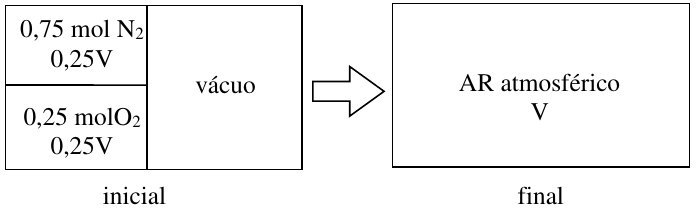
\includegraphics[width=0.5\textwidth]{2021-06-07-07-39-24.png}
        \end{center}

        \begin{parts}
            \part Calcule a variação de entropia do \ce{N2} e do \ce{O2} entre os estados
            final e inicial sabendo que a temperatura permanece constante.
            Indique os cálculos a partir da derivada total apropriada.
            \begin{solution}
                Modelamos a expansão livre dos dois gases no vácuo e a difusão
                de um gás no outro como expansões isotérmicas. Primeiro
                calculamos $\dif Q$ para a expansão isotérmica de um gás ideal:

                \begin{align*}
                    \dif T = 0 \implies \dif U & = \dif Q + \dif w = 0 \\
                    \dif Q & = -\dif w \\
                    \dif Q & = - (-P\dif V) = P\dif V
                \end{align*}

                A partir disso, obtemos a entropia para as duas expansões:

                \begin{multi}

                    De \ce{N2}:

                    \begin{align*}
                        \Delta S_{\ce{N2}} & = \int_i^f \dfrac{\dif Q_{rev}}{T} \\
                        & = \int_i^f \dfrac{P\dif V}{T} \\
                        & = \int_i^f \dfrac{nRT\dif V}{VT} \\
                        & = nR \int_i^f \dfrac{\dif V}{V} \\
                        & = nR\ln\del{\dfrac{V_f}{V_i}} \\
                        & = \num{0,75} \cdot \num{8,3145} \cdot \ln 4 \\
                        & = \num{6,235875} \cdot \ln 4 \\
                        \implies\Delta S_{\ce{N2}} & \approx \SI{8,64}{\joule\per\kelvin}
                    \end{align*}

                    \nextcol

                    E de \ce{O2}:

                    \begin{align*}
                        \Delta S_{\ce{O2}} & = \int_i^f \dfrac{\dif Q_{rev}}{T} \\
                        & = \int_i^f \dfrac{P\dif V}{T} \\
                        & = \int_i^f \dfrac{nRT\dif V}{VT} \\
                        & = nR \int_i^f \dfrac{\dif V}{V} \\
                        & = nR\ln\del{\dfrac{V_f}{V_i}} \\
                        & = \num{0,25} \cdot \num{8,3145} \cdot \ln 4 \\
                        & = \num{2,078625} \cdot \ln 4 \\
                        \implies \Delta S_{\ce{O2}} & \approx \SI{2,88}{\joule\per\kelvin}
                    \end{align*}

                \end{multi}

            \end{solution}
            \part Calcule a variação de entropia total do sistema entre o estado
            inicial e final (após a remoção das divisórias).

            \begin{solution}
                Não há interação com a vizinhança, então a variação total de
                entropia é só a soma das variações de entropia dos dois gases:

                \[\Delta S_{tot} = \num{2,88} + \num{8,64} = \SI{11,52}{\joule\per\kelvin}\]
            \end{solution}

            \part Explique porque a mistura de \ce{O2} e \ce{N2}, nas condições descritas,
            pode ser considerada como um processo adiabático ($\dif q = 0$).

            \begin{solution}
                Os dois gases estão na mesma temperatura ao longo do processo
                todo, então não há troca de calor entre os dois. A parede
                adiabática também previne a troca de calor entre os gases e a
                vizinhança.
            \end{solution}

            \part Algumas vezes os alunos respondem o item a dizendo que a
            variação de entropia é zero pois a entropia é definida como
            $\dif S = \dif q_{rev}/T$ e, sendo o processo adiabático (item c),
            $\dif S$ também deveria ser zero. Explique qual é o problema com
            esse raciocínio.

            \begin{solution}
                A entropia é definida a partir de $\dif Q$ \textbf{reversível}, e a
                expansão livre não é um processo reversível. Isso já basta para
                determinar que $\dif S$ não é 0 (processos irreversíveis tem $\dif S$
                maior que 0).

                Para obter o valor de $\dif S$, é necessário obter $\dif Q$ para um
                processo reversível que leve o sistema do mesmo estado inicial
                para o mesmo estado final que a expansão livre. Esse processo
                não é uma expansão adiabática, mas sim uma expansão
                \textbf{isotérmica}, já que o gás não sofre mudança de
                temperatura.
            \end{solution}

        \end{parts}

        \question Você sabe que a combustão incompleta de combustíveis fósseis
        pode gerar monóxido de carbono e dióxido de carbono, gases importantes
        no efeito estufa tido como responsável pelo aquecimento global. Em
        função disso, o estudo da reação

        \[ \ce{CO}(g) + \ce{H2O}(g) \rightarrow \ce{CO2}(g) + \ce{H2}(g) \]

        é de fundamental importância sob o ponto de vista prático. A partir dos dados
        fornecidos, calcule:

        \begin{parts}
            \part verifique se a reação é favorável a \SI{298}{\kelvin}

            \begin{solution}
                Dada a equação da energia livre de Gibbs:
                \[\Delta G = \Delta H – T\cdot \Delta, S\]
                em que a espontaneidade de uma reação dependerá diretamente de $\Delta G$
                (para $\Delta G < 0$ a reação será espontânea, por aumentar entropia do
                sistema e para  $\Delta G>0$ a reação não será espontânea).

                Sabendo que em $\Delta G = \Delta H – T \cdot \Delta S$, teremos
                $\Delta S = \SI{-42,4}{\joule\per\mole\per\kelvin}$,
                assim como $T = \SI{298}{\kelvin}$, desse modo precisaremos
                calcular $\Delta H$, tal que
                \[\Delta H = \sum \underbrace{\Delta H(f)}_{\text{produtos}} - \underbrace{\sum \Delta H(f)}_{\text{reagentes}}.\]
                Isto é, da reação:
                \[\ce{CO}(g) + \ce{H2O}(g) \rightarrow \ce{CO2}(g) + \ce{H2}(g)\]
                dado que entalpia do gás de hidrogênio é nula, teremos
                \begin{align*}
                    \Delta H &= (\SI{-393,54}{\kilo\joule\per\mole} + 0)
                        - (\SI{-120,52}{\kilo\joule\per\mole}
                        - \SI{241,83}{\kilo\joule\per\mole})\\
                    \Delta H &= (\num{-393,54} + \num{362,35}) = \SI{-32,19}{\kilo\joule\per\mole}.
                \end{align*}

                Logo,
                \begin{align*}
                    \Delta G &= \Delta H – T\cdot \Delta S\\
                    &= \SI{-32,19}{\kilo\joule\per\mole}- \SI{298}{\kelvin} \cdot (\SI{-42,4}{\joule\per\mole\per\kelvin})\\
                    &= \SI{-32,19}{\kilo\joule\per\mole} + \SI{12635,2}{\joule\per\mole}
                \end{align*}
                Ou seja, $\Delta G < 0$, logo a reação será espontânea.
            \end{solution}

            \part determine a temperatura na qual a reação se torna favorável no
            sentido oposto. Considere que apenas o $C_{P,m}$, das espécies envolvidas
            pode ser considerado constante nesse intervalo de temperatura.
            \paragraph{Dados:}
            \begin{gather*}
                \Delta_f H^0_{298}(\ce{CO},g) = \SI{-110,52}{\kilo\joule\per\mole}\\
                \Delta_f H^0_{298}(\ce{H2O},g) = \SI{-241,83}{\kilo\joule\per\mole}\\
                \Delta_f H^0_{298}(\ce{CO2},g) = \SI{-393,54}{\kilo\joule\per\mole}.\\
                \intertext{Para a reação direta:}
                \Delta_r S^0_{298} =\SI{-42,4}{\joule\per\mole\per\kelvin}\\
                C_{P,m}(\SI{298}{\kelvin})(\ce{CO}(g))  = \SI{29,14}{\joule\per\mole\per\kelvin}\\
                C_{P,m}(\SI{298}{\kelvin})(\ce{H2O}(g)) = \SI{33,58}{\joule\per\mole\per\kelvin}\\
                C_{P,m}(\SI{298}{\kelvin})(\ce{CO2}(g)) = \SI{37,11}{\joule\per\mole\per\kelvin}\\
                C_{P,m}(\SI{298}{\kelvin})(\ce{H2}(g))  = \SI{28,82}{\joule\per\mole\per\kelvin}.
            \end{gather*}

            \begin{solution}
                Dada a equação de Kirchhoff, derivamos que
                \[\Delta_r H^0(T_2)=\Delta_rH^0(T_1)+\int_{T_1}^{T_2}\Delta_rC_P^0\dif T.\]

                Em $\ce{CO}(g)+\ce{H2O}+\ce{H2}(g)$.
                \begin{align*}
                    \Delta C_{P,m} &= \underbrace{\sum C_P}_{\text{produtos}} -
                    \underbrace{\sum C_P}_{\text{reagentes}} =
                    C_{P,m}(\SI{298}{\kelvin})\\
                    &= C_{P,\text{reagentes}} -C_{P,\text{produtos}} = ((\num{37,11}+\num{28,82}) - (\num{29,14} + \num{33,58}))\\
                    \Delta C_{P,m}&= \SI{3.21}{\joule\per\mole\per\kelvin}\\
                    &=\Delta_r H^0(T_1) + \Delta_r C_P^0 (T_2-T_1)
                \end{align*}
                Para T1 = 298K
                \[\Delta_rH^0(T_1) = \Delta_rH^0(\SI{298}{\kelvin}) = \SI{-32,19}{\kilo\joule\per\mole}\]
                \[C_{P,m} = \SI{3.21}{\joule\per\mole\per\kelvin}.\]
                Logo,
                \begin{align*}
                    \Delta_r H^0(T_2)&= \SI{-32,19}{\kilo\joule\per\mole} + \SI{3.21}{\joule\per\mole\per\kelvin}(T_2-\SI{298}{\kelvin})\\
                    &= \SI{-32,19}{\kilo\joule\per\mole} - \SI{956,58}{\joule\per\mole} + (\SI{3.21}{\joule\per\mole}) T_2\\
                    &= \SI{-31233.42}{\kilo\joule\per\mole} + (\SI{3.21}{\joule\per\mole}) T_2
                \end{align*}
                dado
                \[\Delta G = \Delta H – T \cdot \Delta S,\]
                temos que $\Delta S = S_{\text{final}} - S_{\text{inicial}} =
                T_1\,T_2C_P\dif T/T$, para $C_P$ constante,
                \[\Delta S  = C_P\,T_1\,T_2\dif T/T= C_P(\ln(T_2) - \ln(T_1)).\]
                Dado, $C_{P,m} = \SI{3.21}{\joule\per\mole\per\kelvin}$, teremos
                que para a situação limite $\Delta G = \Delta H – T\cdot \Delta S = 0$.
                A raiz de $T2$ será a temperatura que estamos procurando, isto é,
                \begin{align*}
                    \Delta G &= \Delta H – T\cdot \Delta S\\
                    &= \SI{-31233.42}{\kilo\joule\per\mole} + (\SI{3.21}{\joule\per\mole})\cdot T_2 -T_2(\SI{3.21}{\joule\per\mole\per\kelvin}(\ln(T_2) - \ln(\SI{298}{\kelvin})) =0
                \end{align*}
                \begin{center}
                    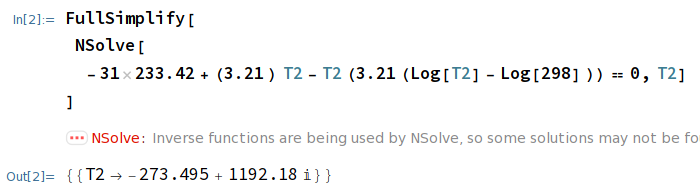
\includegraphics[width=0.8\linewidth]{2021-06-07-17-31-14.png}
                \end{center}

            \end{solution}
        \end{parts}

        \appendix\label{code:math}

        \begin{lstlisting}
\[Alpha][R_, T_, P_] := (R T)/(3 P)

u[R_, T_, P_] := V - \[Alpha][R, T, P]

\[Gamma][R_, T_, P_, B_] := \[Alpha][R, T, P] B - \[Alpha][R, T, P]^2

f := 1/3 u^3 + u \[Gamma] - \[Alpha] C

fn[R_, T_, P_, B_, C_] :=
    1/3 u[R, T, P]^3 +
    u[R, T, P] \[Gamma][R, T, P, B] - \[Alpha][R, T, P] C

FullSimplify[
    Solve[
            {
                fn[R, T, P, B, C]
            } == 0, V
        ]
    ]
{V -> (-6 2^(1/3) B P^5 R T + 2 2^(1/3) P^4 R^2 T^2 +
    2 P^2 R T (27 C P^8 R T + Sqrt[
    P^12 R^2 T^2 (729 C^2 P^4 - 4 R T (-3 B P + R T)^3)])^(1/3) +
    2^(2/3) (27 C P^8 R T + Sqrt[
    P^12 R^2 T^2 (729 C^2 P^4 - 4 R T (-3 B P + R T)^3)])^(
    2/3))/(6 P^3 (27 C P^8 R T + Sqrt[
    P^12 R^2 T^2 (729 C^2 P^4 - 4 R T (-3 B P + R T)^3)])^(1/3))}

FullSimplify[
    NSolve[
        {((-6 2^(1/3) B P^5 R T + 2 2^(1/3) P^4 R^2 T^2 +
            2 P^2 R T (27 C P^8 R T + \[Sqrt](P^12 R^2 T^2 (729 C^2 P^4 \
            - 4 R T (-3 B P + R T)^3)))^(1/3) +
            2^(2/3) (27 C P^8 R T + \[Sqrt](P^12 R^2 T^2 (729 C^2 P^4 -
            4 R T (-3 B P + R T)^3)))^(
            2/3))/(6 P^3 (27 C P^8 R T + \[Sqrt](P^12 R^2 T^2 (729 C^2 \
            P^4 - 4 R T (-3 B P + R T)^3)))^(1/3)))/(R T/P) == Z} /. {
                T -> 273,
                R -> 0.082057,
                B -> -21.7,
                C -> 1200
                }, Z]]
{Z -> (9.40807 P^4 + 27.3403 P^5 +
    0.333333 P^2 (725811. P^8 +
    22.4016 \[Sqrt](P^12 (1.04976*10^9 P^4 -
    2.47219*10^7 (0.34411 + 1. P)^3)))^(1/3) +
    0.0118102 (725811. P^8 +
    22.4016 \[Sqrt](P^12 (1.04976*10^9 P^4 -
    2.47219*10^7 (0.34411 + 1. P)^3)))^(
    2/3))/(P^2 (725811. P^8 +
    22.4016 \[Sqrt](P^12 (1.04976*10^9 P^4 -
    2.47219*10^7 (0.34411 + 1. P)^3)))^(1/3))}

NSolve[
    {Z == (9.408066084801346` P^4 + 27.340286782718742` P^5 +
        0.3333333333333333` P^2 (725810.5764` P^8 +
        22.401561` \[Sqrt](P^12 (1.04976`*^9 P^4 -
        2.472186549455204`*^7 (0.34411` + 1.` P)^3)))^(1/3) +
        0.011810196708823098` (725810.5764` P^8 +
        22.401561` \[Sqrt](P^12 (1.04976`*^9 P^4 -
        2.472186549455204`*^7 (0.34411` + 1.` P)^3)))^(
        2/3))/(P^2 (725810.5764` P^8 +
        22.401561` \[Sqrt](P^12 (1.04976`*^9 P^4 -
        2.472186549455204`*^7 (0.34411` + 1.` P)^3)))^(
        1/3))} /. {P -> 100*101325/100^2}]
{Z -> 137.661}
        \end{lstlisting}

    \end{questions}
\end{document}
